\documentclass[11pt]{article}
\usepackage{hyperref}
\usepackage{graphicx}
\usepackage{amssymb}
\usepackage[fleqn]{amsmath}
\usepackage{epstopdf}
\usepackage{mathrsfs}
\usepackage{mdframed}
\DeclareGraphicsRule{.tif}{png}{.png}{`convert #1 `dirname #1`/`basename #1 .tif`.png}
\usepackage[noline, boxed, titlenotnumbered, linesnumberedhidden]{algorithm2e}

\textwidth = 6.5 in
\textheight = 9 in
\oddsidemargin = 0.0 in
\evensidemargin = 0.0 in
\topmargin = 0.0 in
\headheight = 0.0 in
\headsep = 0.0 in
\parskip = 0.2in
\parindent = 0.0in

\newtheorem{theorem}{Theorem}
\newtheorem{corollary}[theorem]{Corollary}
\newtheorem{definition}{Definition}

\title{Brief Article}
\author{The Author}
\begin{document}
%\maketitle

\section*{Zeroing $\hat{\beta_i}$ in low-dimensional feature space}

{\bf Q}. Why does L1 make it easy to get at least one $\hat{\beta_i}=0$?

{\bf Preliminary 1}. My argument hinges on the fact that the minimum MSE loss point, for a non-spherical ellipsoid, falls on the line along the major axis, which we can call the {\em min line}:

\begin{center}
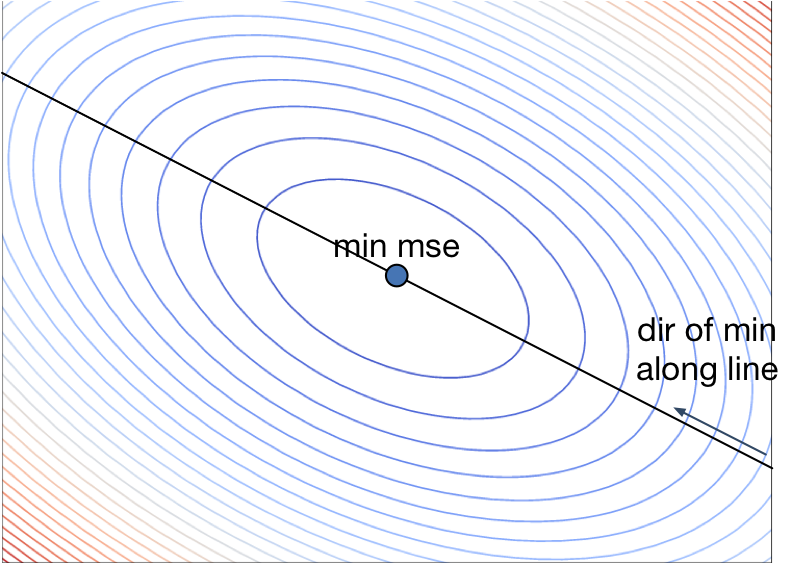
\includegraphics[scale=.5]{images/min-line.png}
\end{center}

\noindent While the ellipsoid cross-sections (levels looking down from above) have equal MSE, the minimum MSE is a point and it falls on the major axis line.

{\bf Preliminary 2}. We are optimizing ${\mathscr L}(\beta, t)$ or ${\mathscr L}(\beta, \lambda)$ with another hyperparameter.  Let's stick with $t$ from the inequality ``hard constraint'' version of regularization. That means we can choose $t$ to be anything we want.

{\bf Q}. Does L1 regularization encourage $\hat{\beta_i}=0$ coefficient estimates for $\hat{\beta} = (\hat{\beta_1}, \hat{\beta_2})$?

{\bf A}. Yes. David U explained.

\end{document}